\documentclass[12pt]{article}
% REVISION NOTES %%%%%%%%%%%%%%%%%%%%%%%%%%%%%%%%%%%%%%%%%%%%
% 2008-0814 Location, Date, Time
% 2008-0814 fixed citations -- added bibliography.
%
%
\usepackage{geometry}                
\geometry{letterpaper}                   
%\geometry{landscape}                
\usepackage[parfill]{parskip}    
\usepackage{daves,fancyhdr,natbib,graphicx,dcolumn,amsmath,lastpage,url}
\usepackage{amsmath,amssymb,epstopdf,longtable}
\usepackage{caption}
\usepackage{subcaption}
\usepackage[final]{pdfpages}
\DeclareGraphicsRule{.tif}{png}{.png}{`convert #1 `dirname #1`/`basename #1 .tif`.png}
\pagestyle{fancy}
\lhead{CE 3105 -- Fluid Mechanics Laboratory}
\rhead{FALL 2023}
\lfoot{CE 3105 -- Cleveland}
\cfoot{Page \thepage\ of \pageref{LastPage}}
\rfoot{REVISED: 27 NOV 2023}
\renewcommand\headrulewidth{0pt}
%%%%%%%%%%%%%%%%%%%%%%%%%%%%%%%%%%%%%%%%%%%%%%%%%%%%%%%%%%%%%%%%%%%%%%%%%%%%%%%%%%%%
\begin{document}
\section*{\center{ { CE 3105 -- Fluid Mechanics Laboratory} {Final Exam} } }
\begin{itemize}
\item Please read through the entire exam before you begin - notice there are blank pages to show your work, so make it legible and follow a logical problem solving protocol.
\item Write your name on \textbf{each} sheet before beginning to work the exam.
\end{itemize}
%%%%%%%%%%%%%%%%%%%%%%%%%%%%%%%%%%%%%%%%%%%%%%%%%%%%%%%%%%%%%%%%%%%%%%%%%%%%%%%%%%%%
\section*{Question 1}
What are the names of your laboratory team members:
\begin{enumerate}
\item TEAM MEMBER 0 (YOU): $\underline{~~~~~~~~~~~~~~~~~~~~~~~~~~~~~~~~~~~~~~~~}$
\item TEAM MEMBER 1: $\underline{~~~~~~~~~~~~~~~~~~~~~~~~~~~~~~~~~~~~~~~~~~~~~~}$
\item TEAM MEMBER 2: $\underline{~~~~~~~~~~~~~~~~~~~~~~~~~~~~~~~~~~~~~~~~~~~~~~}$
\item TEAM MEMBER 3: $\underline{~~~~~~~~~~~~~~~~~~~~~~~~~~~~~~~~~~~~~~~~~~~~~~}$
\item TEAM MEMBER 4: $\underline{~~~~~~~~~~~~~~~~~~~~~~~~~~~~~~~~~~~~~~~~~~~~~~}$
\item TEAM MEMBER 5: $\underline{~~~~~~~~~~~~~~~~~~~~~~~~~~~~~~~~~~~~~~~~~~~~~~}$
\end{enumerate}
\clearpage
%%%%%%%%%%%%%%%%%%%%%%%%%%%%%%%%%%%%%%%%%%%%%%%%%%%%%%%%%%%%%%%%%%%%%%%%%%%%%%%%%%%%
\section*{Question 2}
Before each laboratory you received a safety briefing.  What were three safety reminders before each laboratory?
\begin{enumerate}
\item REMINDER 1: $\underline{~~~~~~~~~~~~~~~~~~~~~~~~~~~~~~~~~~~~~~~~~~~~~~~~~~~~~~~~~~~~~~~~~~~~~~~~~~~}$
\item REMINDER 2: $\underline{~~~~~~~~~~~~~~~~~~~~~~~~~~~~~~~~~~~~~~~~~~~~~~~~~~~~~~~~~~~~~~~~~~~~~~~~~~~}$
\item REMINDER 3: $\underline{~~~~~~~~~~~~~~~~~~~~~~~~~~~~~~~~~~~~~~~~~~~~~~~~~~~~~~~~~~~~~~~~~~~~~~~~~~~}$
\end{enumerate}
%%%%%%%%%%%%%%%%%%%%%%%%%%%%%%%%%%%%%%%%%%%%%%%%%%%%%%%%%%%%%%%%%%%%%%%%%%%%%%%%%%%%
\clearpage
\section*{Question 3}
A metal sphere measured using a dial-caliper (in inches) is pictured. The same sphere is weighed using a digital scale (in grams). 
\begin{figure}[h!] %  figure placement: here, top, bottom, or page
   \centering
   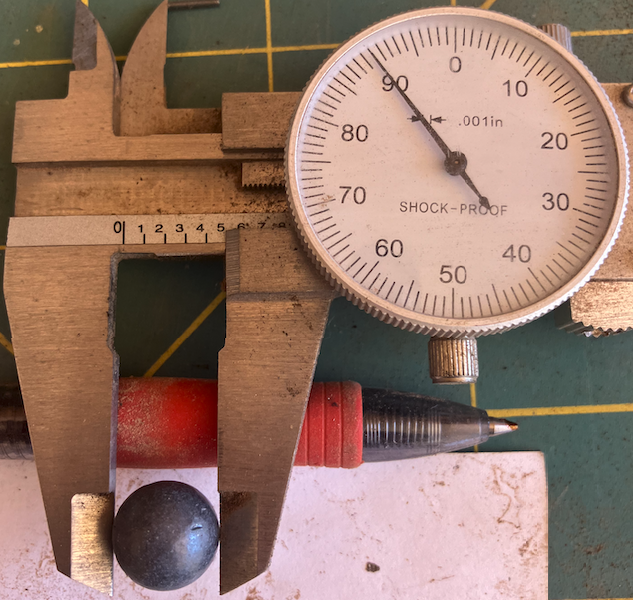
\includegraphics[width=2.75in]{sphere-dimension.png} 
   \caption{Sphere in dial-caliper instrument reading diameter in inches}
   \label{fig:sphere-dimension}
\end{figure}

\begin{figure}[h!] %  figure placement: here, top, bottom, or page
   \centering
   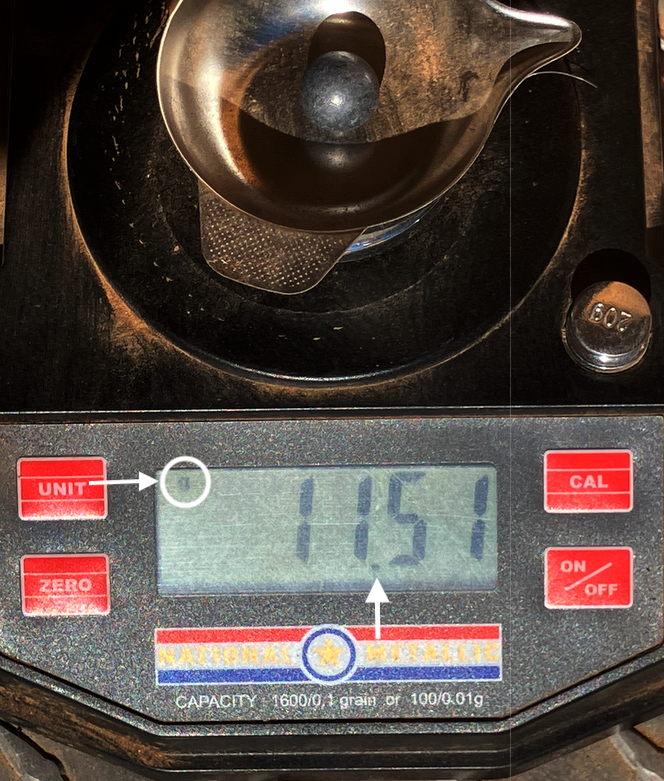
\includegraphics[width=2.75in]{sphere-mass.png} 
   \caption{Sphere on scale reading mass in grams}
   \label{fig:sphere-mass}
\end{figure}
\newpage
Determine:
\begin{enumerate}
\item The volume of the sphere in milliliters
\item The density of the sphere in $\frac{g}{ml}$
\end{enumerate}
\clearpage
Show work here
\clearpage
\section*{Question 4}
The sphere (color coated for visibility) is used to estimate viscosity for an unknown liquid as depicted in the photographs below. A 50 ml sample of the light amber liquid has a mass of 69.5 grams at 20$^o$C. The time required for the sphere to traverse 127 mm was observed to be 2.3 seconds.
\begin{figure}[h!]
\centering
\begin{subfigure}{.3\textwidth}
  \centering
  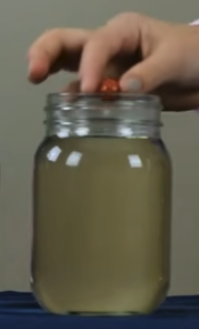
\includegraphics[width=.4\linewidth]{drop.png}
  \caption{Dropping sphere}
  \label{fig:sub1}
\end{subfigure}%
\begin{subfigure}{.3\textwidth}
  \centering
  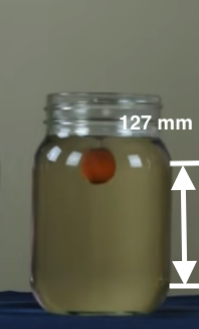
\includegraphics[width=.4\linewidth]{begin.png}
  \caption{Time = 0 sec.}
  \label{fig:sub2}
\end{subfigure}
\begin{subfigure}{.3\textwidth}
  \centering
  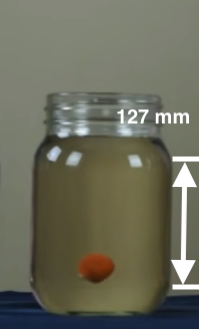
\includegraphics[width=.4\linewidth]{end.png}
  \caption{Time = 2.3 sec.}
  \label{fig:sub2}
\end{subfigure}
\caption{Spherical object for viscosity measurement by Stokes Law (Laboratory 1)}
\label{fig:test}
\end{figure}
Determine:
\begin{enumerate}
\item The density of the unknown liquid (in $\frac{g}{ml}$)
\item The viscosity of the unknown liquid (in Pa$\cdot$s)
\end{enumerate}
\clearpage
Show work here
\clearpage
\section*{Question 5}
The following discharge data and head change were obtained using the apparatus in the photograph below:

\begin{table}[h!]
    \centering
    \caption{Pipe head loss apparatus (Laboratory 4)}
    \begin{tabular}{p{1in} p{1in} p{1in}}
    Volume (mL) & Time (s) & $\Delta h$ (m) \\
    \hline
    122&8.36&1.34\\
    138&6.67&2.56\\
    180&7.9&3.09\\
    205&8.03&3.98\\
    217&8.26&3.92\\
    \end{tabular}
    \label{tab:table1}
\end{table}

\begin{figure}[h!] %  figure placement: here, top, bottom, or page
   \centering
   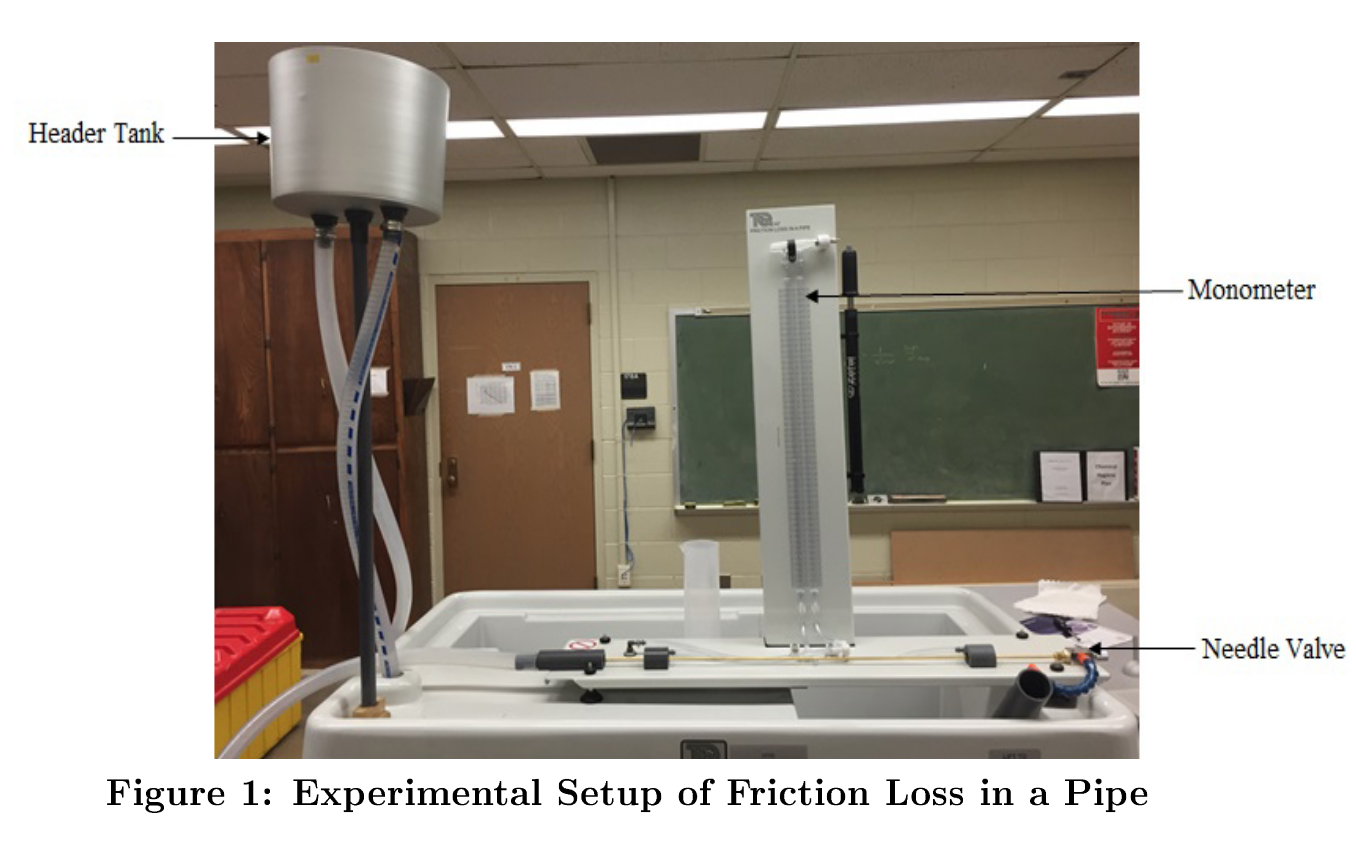
\includegraphics[width=4in]{labsetup.png} 
   \caption{Pipe head loss apparatus (Laboratory 4)}
   \label{fig:labsetup}
\end{figure}

Determine:
\begin{enumerate}
\item The discharge rate for each of the 5 measurements.
\item The flow velocity in the 3-mm brass tube for each of the 5 measurements.
\item The Reynolds number for each of the 5 measurements.
\item The Darcy-Weisbach friction factor for each of the 5 measurements.
\item The flow regime (laminar, transitional, or turbulent) in each experiment?
\item Plot (sketch) the friction factor versus Reynolds number for these data.
\end{enumerate}
\clearpage
Show work here
\clearpage
Show work here
\clearpage
%%%%%%%%%%%%%%%%%%%%%%%%%%%%%%%%%%%%%%%%%%%%%%%%%%%%%%%%%%%%%%%%%%%%%%%%%%%%%%%%%%%%
\bibliographystyle{chicago}	         % (uses file "chicago.bst")
\end{document}

\begin{figure}[h!] %  figure placement: here, top, bottom, or page
   \centering
   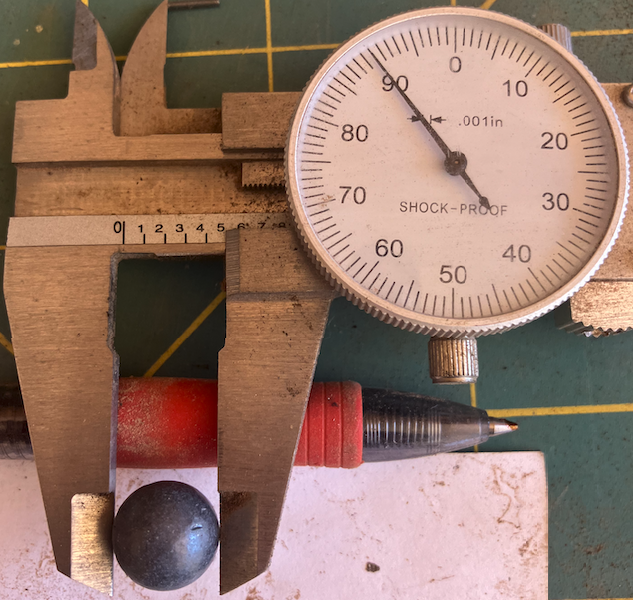
\includegraphics[width=3in]{sphere-dimension.png} 
   \caption{Sphere in dial-caliper instrument reading diameter in inches}
   \label{fig:sphere-dimension}
\end{figure}
\begin{figure}[h!] %  figure placement: here, top, bottom, or page
   \centering
   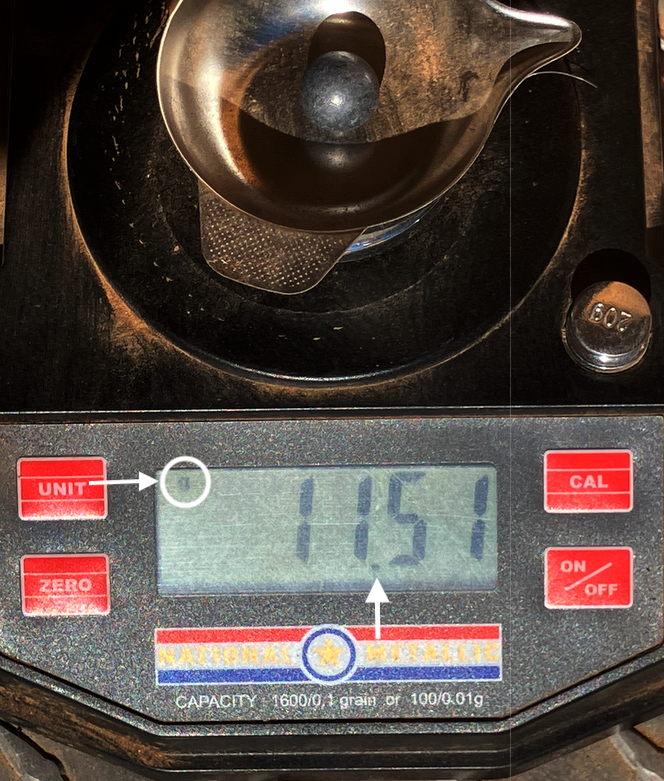
\includegraphics[width=3in]{sphere-mass.png} 
   \caption{Sphere on scale reading mass in grams}
   \label{fig:sphere-mass}
\end{figure}

\begin{figure}
\centering
\begin{subfigure}{.5\textwidth}
  \centering
  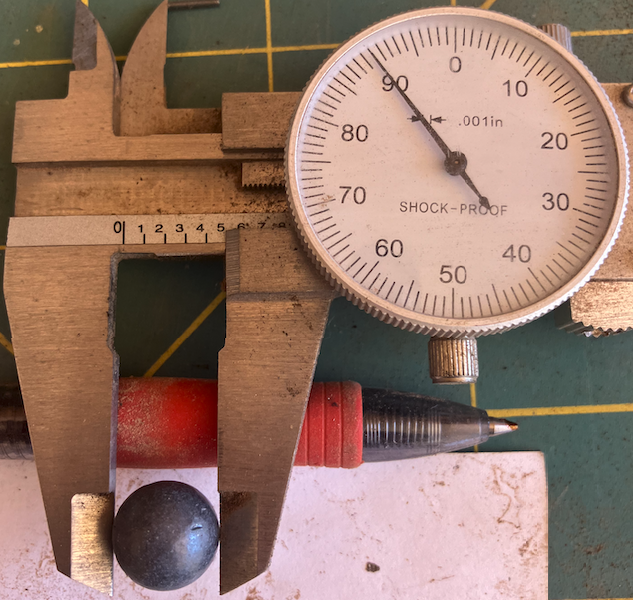
\includegraphics[width=.4\linewidth]{sphere-dimension.png}
  \caption{Sphere in dial-caliper instrument reading diameter in inches}
  \label{fig:sub1}
\end{subfigure}%
\begin{subfigure}{.5\textwidth}
  \centering
  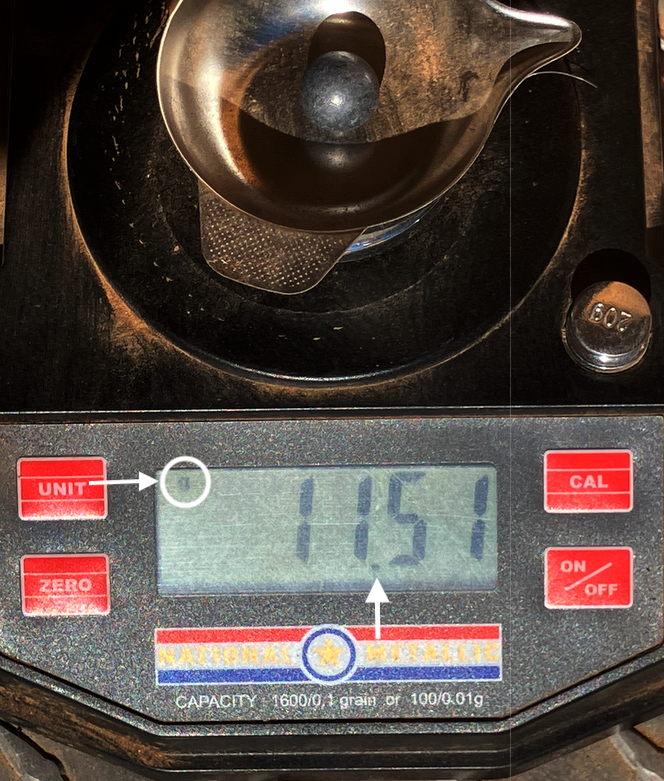
\includegraphics[width=.4\linewidth]{sphere-mass.png}
  \caption{Sphere on scale reading mass in grams}
  \label{fig:sub2}
\end{subfigure}
\caption{Photographs of spherical object for viscosity measurement}
\label{fig:test}
\end{figure}

\begin{figure}[h!] %  figure placement: here, top, bottom, or page
   \centering
   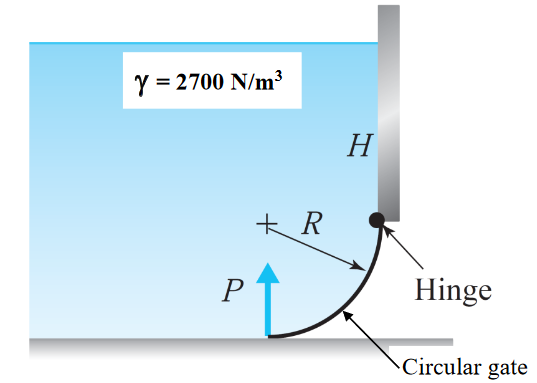
\includegraphics[width=3in]{circlegate.png} 
   \caption{}
   \label{fig:circlegate}
\end{figure}